% A LaTeX (non-official) template for ISAE projects reports
% Copyright (C) 2014 Damien Roque
% Version: 0.2
% Author: Damien Roque <damien.roque_AT_isae.fr>

\documentclass[a4paper,12pt]{book}
\usepackage[utf8]{inputenc}             % The input file is in utf-8
\usepackage{marvosym}                   % This package provides some symbols. The € is 
\DeclareUnicodeCharacter{20AC}{\EUR{}} 
\usepackage[utf8]{inputenc}
\usepackage[T1]{fontenc}
\usepackage[frenchb]{babel} % If you write in French
%\usepackage[english]{babel} % If you write in English
\usepackage{a4wide}
\usepackage{graphicx}
\graphicspath{{images/}}
\usepackage{subfig}
\usepackage{tikz}
\usepackage{float} 
\usetikzlibrary{shapes,arrows}
\usepackage{pgfplots}
\pgfplotsset{compat=newest}
\pgfplotsset{plot coordinates/math parser=false}
\newlength\figureheight
\newlength\figurewidth
\pgfkeys{/pgf/number format/.cd,
set decimal separator={,\!},
1000 sep={\,},
}
\usepackage{ifthen}
\usepackage{ifpdf}
\ifpdf
\usepackage[pdftex]{hyperref}
\else
\usepackage{hyperref}
\fi
\usepackage{color}
\hypersetup{%
colorlinks=true,
linkcolor=black,
citecolor=black,
urlcolor=black}

\renewcommand{\baselinestretch}{1.05}
\usepackage{fancyhdr}
\pagestyle{fancy}
\fancyfoot{}
\fancyhead[LE,RO]{\bfseries\thepage}
\fancyhead[RE]{\bfseries\nouppercase{\leftmark}}
\fancyhead[LO]{\bfseries\nouppercase{\rightmark}}
\setlength{\headheight}{15pt}

\let\headruleORIG\headrule
\renewcommand{\headrule}{\color{black} \headruleORIG}
\renewcommand{\headrulewidth}{1.0pt}
\usepackage{colortbl}
\arrayrulecolor{black}

\fancypagestyle{plain}{
  \fancyhead{}
  \fancyfoot[C]{\thepage}
  \renewcommand{\headrulewidth}{0pt}
}

\makeatletter
\def\@textbottom{\vskip \z@ \@plus 1pt}
\let\@texttop\relax
\makeatother

\makeatletter
\def\cleardoublepage{\clearpage\if@twoside \ifodd\c@page\else%
  \hbox{}%
  \thispagestyle{empty}%
  \newpage%
  \if@twocolumn\hbox{}\newpage\fi\fi\fi}
\makeatother

\usepackage{amsthm}
\usepackage{amssymb,amsmath,bbm}
\usepackage{array}
\usepackage{bm}
\usepackage{multirow}
\usepackage[footnote]{acronym}

\newcommand*{\SET}[1]  {\ensuremath{\mathbf{#1}}}
\newcommand*{\VEC}[1]  {\ensuremath{\boldsymbol{#1}}}
\newcommand*{\FAM}[1]  {\ensuremath{\boldsymbol{#1}}}
\newcommand*{\MAT}[1]  {\ensuremath{\boldsymbol{#1}}}
\newcommand*{\OP}[1]  {\ensuremath{\mathrm{#1}}}
\newcommand*{\NORM}[1]  {\ensuremath{\left\|#1\right\|}}
\newcommand*{\DPR}[2]  {\ensuremath{\left \langle #1,#2 \right \rangle}}
\newcommand*{\calbf}[1]  {\ensuremath{\boldsymbol{\mathcal{#1}}}}
\newcommand*{\shift}[1]  {\ensuremath{\boldsymbol{#1}}}

\newcommand{\eqdef}{\stackrel{\mathrm{def}}{=}}
\newcommand{\argmax}{\operatornamewithlimits{argmax}}
\newcommand{\argmin}{\operatornamewithlimits{argmin}}
\newcommand{\ud}{\, \mathrm{d}}
\newcommand{\vect}{\text{Vect}}
\newcommand{\sinc}{\ensuremath{\mathrm{sinc}}}
\newcommand{\esp}{\ensuremath{\mathbb{E}}}
\newcommand{\hilbert}{\ensuremath{\mathcal{H}}}
\newcommand{\fourier}{\ensuremath{\mathcal{F}}}
\newcommand{\sgn}{\text{sgn}}
\newcommand{\intTT}{\int_{-T}^{T}}
\newcommand{\intT}{\int_{-\frac{T}{2}}^{\frac{T}{2}}}
\newcommand{\intinf}{\int_{-\infty}^{+\infty}}
\newcommand{\Sh}{\ensuremath{\boldsymbol{S}}}
\newcommand{\C}{\SET{C}}
\newcommand{\R}{\SET{R}}
\newcommand{\Z}{\SET{Z}}
\newcommand{\N}{\SET{N}}
\newcommand{\K}{\SET{K}}
\newcommand{\reel}{\mathcal{R}}
\newcommand{\imag}{\mathcal{I}}
\newcommand{\cmnr}{c_{m,n}^\reel}
\newcommand{\cmni}{c_{m,n}^\imag}
\newcommand{\cnr}{c_{n}^\reel}
\newcommand{\cni}{c_{n}^\imag}
\newcommand{\tproto}{g}
\newcommand{\rproto}{\check{g}}
\newcommand{\LR}{\mathcal{L}_2(\SET{R})}
\newcommand{\LZ}{\ell_2(\SET{Z})}
\newcommand{\LZI}[1]{\ell_2(\SET{#1})}
\newcommand{\LZZ}{\ell_2(\SET{Z}^2)}
\newcommand{\diag}{\operatorname{diag}}
\newcommand{\noise}{z}
\newcommand{\Noise}{Z}
\newcommand{\filtnoise}{\zeta}
\newcommand{\tp}{g}
\newcommand{\rp}{\check{g}}
\newcommand{\TP}{G}
\newcommand{\RP}{\check{G}}
\newcommand{\dmin}{d_{\mathrm{min}}}
\newcommand{\Dmin}{D_{\mathrm{min}}}
\newcommand{\Image}{\ensuremath{\text{Im}}}
\newcommand{\Span}{\ensuremath{\text{Span}}}

\newtheoremstyle{break}
  {11pt}{11pt}%
  {\itshape}{}%
  {\bfseries}{}%
  {\newline}{}%
\theoremstyle{break}

%\theoremstyle{definition}
\newtheorem{definition}{Définition}[chapter]

%\theoremstyle{definition}
\newtheorem{theoreme}{Théorème}[chapter]

%\theoremstyle{remark}
\newtheorem{remarque}{Remarque}[chapter]

%\theoremstyle{plain}
\newtheorem{propriete}{Propriété}[chapter]
\newtheorem{exemple}{Exemple}[chapter]

\parskip=5pt
%\sloppy

\begin{document}
\let\cleardoublepage\clearpage
%%%%%%%%%%%%%%%%%%
%%% First page %%%
%%%%%%%%%%%%%%%%%%


\begin{titlepage}
\begin{center}
\vfill

{\large Université de Paris Ouest Nanterre La Défense}\\[0.5cm]

{\large Mémoire}\\[0.5cm]



% Title
\rule{\linewidth}{0.5mm} \\[0.4cm]
{ \huge \bfseries Générateur du code automatique d’après une Modélisation DOMIS \\[0.4cm] }
\rule{\linewidth}{0.5mm} \\[1.5cm]

\vfill
\vfill
\vfill

% Author and supervisor
\noindent
\begin{minipage}{0.7\textwidth}
  \large
    \emph{Réalisé par :}\\
- Nadia \textsc{MASLOUHI}\\
\end{minipage}%
\begin{minipage}{0.5\textwidth}
   \large
    \emph{Encadrants :} \\
- Mme.~Castillo Marta \textsc{RUKOZ}
\end{minipage}

\vfill
\vfill
\vfill
\vfill
\vfill
\vfill
% Bottom of the page

\end{center}
\end{titlepage}
\clearpage


%%%%%%%%%%%%%%%%%%%%%%%%%%%%%%%%%%%%%%%%%%%%
%%% Content of the report and references %%%
%%%%%%%%%%%%%%%%%%%%%%%%%%%%%%%%%%%%%%%%%%%%

\mainmatter
\pagestyle{fancy}





\title{La mise en place d'un générateur du code automatique d’après une Modélisation DOMIS}

\author{nadia.maslouhi }


\section{Introduction}

\vspace{1cm}
B-ADSC (Bucki – Analyse décisionnelle des Systèmes complexes )  est une méthode dédiée à la conception et à l’analyse des systèmes et des organisations qui se base sur l’approche décisionnelle.

L'approche décisionnelle des systèmes complexes consiste en la conception, l'analyse et l'optimisation d'une organisation de telle sorte que les savoir-faire et les procédés employés puissent s’exprimer avec le plus d'efficacité et en totale convergence de buts avec la finalité de l'ensemble.

\vspace{0,5cm}

L'analyse décisionnelle des systèmes complexes met l'accent sur la capacité des organisations pour prendre des décisions sur le pilotage des processus. 
Cet conception se base principalement sur la fixation du but principal et l’élaboration des décisions d’une manière intelligente tout en contrôlant leur évolution afin de les amener à une situation en accord avec l’objectif initial.

\vspace{0,5cm}

Pour B-ADSC, une organisation correspond à une hiérarchie opérationnelle d’activités dans laquelle chaque activité représente « un centre élémentaire de prise de décision » pouvant être piloté par un homme ou par une machine.

Une activité est chargée du pilotage (régulation) du processus en fonction des objectifs qui lui sont assignés par l'environnement.

L'activité contrôle et valide l'évolution du processus, elle-même restant sous le contrôle du niveau supérieur.  Elle assume deux fonctions fondamentales : la décision et le contrôle, et elle communique avec son entourage au moyen de différents flux d’informations.

\vspace{0,5cm}

Une fois la conception est définie, une modélisation des processus sera nécessaire pour administrer les processus et les optimiser pour chacune des activités qui constitue la hiérarchie de B-ADSC.
Pour ce type de modélisation il existe l’outil DOMIS.

DOMIS permet de documenter les processus, il propose un langage générique fondé sur une vision renouvelée de l’organisation.\cite{domis}

Une organisation correspond ici à une hiérarchie opérationnelle d’activités dans laquelle chaque activité représente un « centre élémentaire de prise des décisions ».

DOMIS est l’outil qui permet de définir et modéliser chaque activité en définissant sa fonction de décision et sa fonction d’évolution et les flux d’informations nécessaires.

\vspace{0,5cm}

Après une conception B-ADSC et une modélisation avec l’outil DOMIS l’étape de réalisation et de développement du code correspondant au résultat de la modélisation obtenue peut commencer ; Et c’est là qu’intervient mon sujet de mémoire qui consiste la mise en place d’une solution qui permet la génération du code ‘JAVA’ d’une façon automatique d’après le modèle réalisé sur DoMIS.

\vspace{0,5cm}

D’après le stage effectué en Master 1 qui consiste à la contribution du développement d’une application mobile dont sa conception est basée sur B-ADSC et sa modélisation est basée sur DOMIS, j’ai constaté que la phase qui consiste le passage depuis la modélisation vers le code correspondant, prend beaucoup de temps et rencontre souvent des problèmes dû à la mauvaise interprétation du modèle réalisé sur DOMIS.

La mise en place d’une telle solution va répondre à un vrai besoin pour les développeurs des applications basées sur une modélisation DOMIS, ce besoin a été observé réellement lors du Stage M1 au sein de l’entreprise, et discuté pour essayer de trouver une solution tout en évitant les obstacles rencontrés.

\vspace{0,5cm}

Jusqu’à présent il n’existe aucune solution qui répond à ce besoin, donc la réalisation consiste tout d’abord d'effectuer une étude sur le concept B-ADSC et sur son outil de modélisation DOMIS, ensuite commencer par chercher la méthodologie et les outils nécessaires à la création de ce générateur de code automatique, et finalement entamer la partie développement qui consiste la création de ce dernier.

La solution proposée peut être valider en la testant sur une partie de modélisation de l’application mobile ‘KOOPT’ qui est déjà modélisé sur DOMIS au sein de l’entreprise GLOOKAL.

\vspace{0,5cm}

Pour conclure, je vois que ma solution répond à un vrai besoin actuel qui consiste d’avoir un code généré automatiquement après une modélisation par DOMIS, et ça permet de gagner beaucoup de temps dans la phase de la réalisation d’un projet et d’éviter de nombreux problèmes et bugs qui sont causés la plupart du temps par la mauvaise traduction de la modélisation vers son code correspondant.


\vspace{1cm}

\chapter{État de l'art}

\section{Introduction}

Ce chapitre présente l'étude existante avec son ensemble d'approches pour une exécution fiable des services Web composites.
Cet étude consiste l'exécution auto-corrective (self-healing) d'une manière dynamique et automatique, elle vise le même objectif de ce mémoire mais les méthodologies changent. 

Dans cette étude les chercheurs ont proposé l'approche de l'auto-corrective  (self-healing) qui se base sur les propriétés transactionnelles comme un concept de base pour une tolérance aux pannes automatique, et se base aussi sur les agents à base de connaissances.

Dans un premier temps les auteurs ont proposé une approche pour l'exécution tolérante aux pannes des services Web composite basée sur la récupération en avant et en arrière, et définie par le formalisme de réseaux de Petri Colorés, ensuite sur le même formalisme la deuxième approche consiste la proposition d'un mécanisme de point de contrôle, et finalement après une étude sur l'impact des différentes stratégies de récupération sur les services Web composite, la troisième approche apporte un modèle de décision dynamique de la stratégie de récupération en terme d'impact sur la qualité de service pour la tolérance aux pannes de services Web composites.


\section{Contrôle d'exécution de services Web composites}

En utilisant les réseaux de Petri Colorés les auteurs ont formalisé les services Web composites, leur exécution, et leurs stratégies de tolérance aux pannes, et il ont proposé un framework pour une exécution distribuée fiable et tolérante aux pannes pour les services Web Composites.

Le framework est composé de deux types de composants \cite{1} \cite{5}: 

- Un Coordinateur d'Agents : Composant responsable de la gestion des aspects globaux d'exécution des services Web composites.

- Agents de Service : ils exécutent les services et sont en charge du contrôle de l'exécution et de la tolérance au pannes.

Cette approche fournis les mécanismes de récupération en arrière par compensation, en avant par re-exécution de service et remplacement, la réplication, et le checkpointing, et assure une exécution tolérante aux pannes basé sur un modèle d'exécution distribué.

L'exécution des services Web composite peut être \cite{3} : 

- Séquentiel : Les services se basent sur les résultat des services précédents, et ne peuvent être invoqués tant que les services précédent ne sont pas terminés.

- Parallèle : Les services peuvent être invoqués d'une manière simultanée, car il n'y a pas des dépendances de flux de données entre eux.

Ces deux scénarios d'exécution ont un effet sur la propriété transactionnelle globale du service Web composite, pour cela il faut suivre le flux d'exécution défini par le graphe du service composite pour s'assurer que l'exécution séquentielle et parallèle satisfont la propriété transactionnelle globale.

\subsection{Architecture du Framework}

Les chercheurs ont proposé un Framework dont l'exécution du service composite est gérée par un Coordinateur d'Agents et une collection d'Agents de services, organisés dans architecture trois tiers.

\begin{figure}[H]
\begin{center}
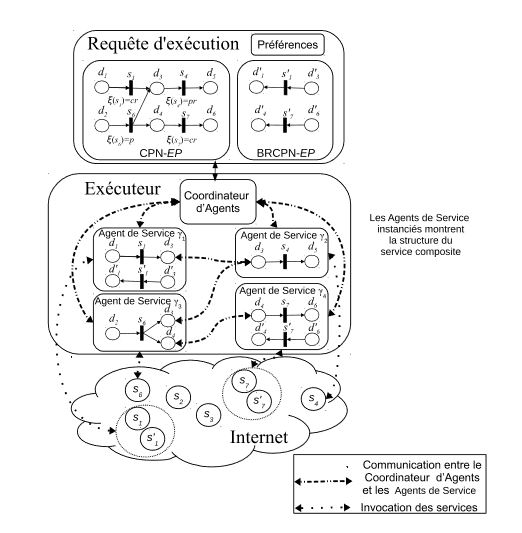
\includegraphics[width=1\linewidth]{images/architectureFrmwork.jpg}
\end{center}
\caption{Architecture d'exécution \cite{1}}
\label{fig:4}
\end{figure}


L’architecture du Framework est composée de trois niveaux principaux:

Le premier niveau : Le coordinateur d’agents reçoit le service composite et son graphe de compensation correspondant, qui sont représentés sous forme des réseau de Pétri Colorés, qui peuvent être générés d'une manière automatique ou manuelle.
Dans ce niveau le Coordinateur reçoit aussi une propriété qui lui indique si le mécanisme de checkpointing est activé ou non.

Le deuxième niveau: Le coordinateur d'Agents lance un Agent de Service pour chaque service composant du service Web composite, chaque agent de service sera responsable du contrôle de l'exécution de son service, ses rôles sont les suivants \cite{1}:

    - Responsabilité de l'invocation de services ;

    - Surveillance de l'exécution des services correspondants ;
    
    - Envoi des résultat selon le flux d'exécution ;
    
    - Lancement des stratégies de tolérance aux pannes en cas de panne.

Le troisième niveau : consiste l'interaction des agents de services avec l'ensemble des services correspondants.

L'objectif de cet architecture est de répartir la responsabilité de l'exécution d'un service Web composite à travers de plusieurs agents de service, pour que le modèle logique de l'exécuteur proposé permet une exécution distribuée et une indépendance de la mise en oeuvre 

\section{Modélisation des stratégies de récupération basées sur QoS}

Après les évolutions des recherches, les auteurs ont découvert a travers leur étude qu'il y a des impacts des différentes stratégies de récupération sur les services Web composite et plus précisément sur sa qualité de service (QoS). C'est pour cela ils ont décidé de proposer une approche pour une décision dynamique des stratégies de récupération.

Pour fournir un choix dynamique de la stratégie de tolérance aux pannes, les auteurs ont proposé une approche auto-corrective (Self-Healing) pour les services Web composites.
Dans l'auto-correctif les agents de services sont des agents basés sur des connaissances, c'est à dire ils sont basés sur l'ensemble des information qu'ils ont sur le service Web composite, sur eux mêmes, et sur ce qui est attendu et ce qu'il se passe réellement pendant l'exécution, pour qu'ils puissent finalement faire la sélection de la stratégie de tolérance aux pannes.

Indépendamment de la technique utilisée pour l'estimation des critères de Qualité de service,ils ont proposé que chaque service Web est annoté avec son temps d'exécution estimé, son prix, sa réputation et sa propriété transactionnelle. Grâce aux critères des services composants, il est possible de calculer la Qualité de service d'un service Web composite en calculant des différents critères.

Sur cette base, la conception sera sous forme d'une boucle d'auto-guérison/auto-correction par agent de service pour effectuer la détection, le diagnostic et la récupération d'une manière décentralisée \cite{1}.


\begin{figure}[H]
\begin{center}
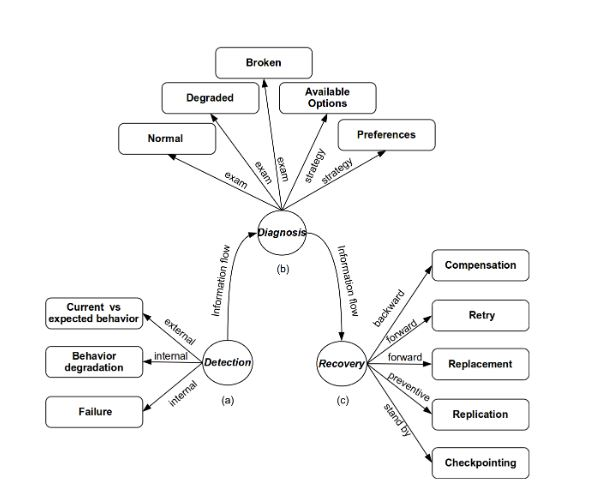
\includegraphics[width=1\linewidth]{images/Boucleauto-correctivedesAgentsdeService.jpg}
\end{center}
\caption{Architecture d'exécution \cite{1}}
\label{fig:5}
\end{figure}

- Le composant detection : Dans ce composant, trois sources sont prises en compte une externe et deux internes. 
La source externe consiste l'information sur la Qualité de service attendu, par exemple, le cas où l'utilisateur peut permettre une certaine dégradation de la Qos.
La source interne concerne la dégradation de la Qualité de service des services composants (par exemple, les variations négatives dans le temps d'exécution et le prix), et concerne aussi les pannes de services.

- Le composant diagnosis : ce composant a le rôle d'analyse du problème et la détermination de l'état du service.
Il existe trois diagnostics possibles qui correspondent au trois états d'un système auto-correctif : normal ; degraded ; et broken. Le choix de la stratégie de récupération est influencé par les options disponibles ( par exemple, les propriétés transactionnelles, les services de remplacement disponible, etc.), et influencé aussi par les préférences de l'utilisateur (la QoS attendu, le checkpointing, etc).

- Le composant recovery :  Ce composant prend en charge l'exécution des mécanismes de tolérance aux pannes sélectionnés : la récupération vers l'arrière avec la compensation ; la récupération en avant par la reexécution ou remplacement ; la prévention grâce à la réplication ; ou le retardement d'exécution par le checkpointing.



\section{Évaluation expérimentale }

Les chercheurs ont mis leur approche en évaluation expérimentale, et ça par la mise en oeuvre du Framework  en utilisant un cas d'étude qui consiste un scénario et un environnement.
L'observation du cas d'étude a été sur trois systèmes différent :

Système sans tolérance au pannes : c'est un système qui n'a aucun mécanisme de tolérance aux pannes. et dans le cas ou un des services composants tombe en panne, une exception sera générée et l'exécution sera terminé.

Système transactionnel : c'est un système qui se base sur les propriétés transactionnelles des services composants pour prendre les décisions de récupération.

Système auto-correctif :  c'est un système qui se base sur l'ensemble d'information et règle contenu dans les bases de connaissances des agents de services.


Les résultat de l'évaluation expérimentale ont montré : l'importance et la nécessité d'avoir des mécanisme de tolérance aux pannes pour les services Web composite, ainsi que la manière avec laquelle les deux approches des propriétés transactionnelles et l'auto-corrective gèrent les pannes et prennent la décision de récupération.
L'évaluation expérimentale faite pendant cette étude suggère que la combinaison des propriétés transactionnelles avec des capacités d'auto-corrective permet de donner une intelligence aux systèmes d'exécution pour gérer les exigences de haut niveau pour les exécutions de services Web composites avec une intervention humaine minimale\cite{1}.

\section{Conclusion}

Pendant cette étude, les auteurs ont proposé une approche auto corrective pour l'exécution de services Web composite qui se base sur les propriété transactionnelles des services Web composants ainsi que sur une base d'informations sur les Services Web qui se présente principalement dans la Qualité de chaque service QoS.

L'avantage principale de cette étude c'est la mise en oeuvre des mécanismes de d'exécution et de récupération qui sont capables de fonctionner d'une manière automatique, ces mécanismes sont mis en place a travers un Framework qui se base sur des agents de services qui sont en charge du contrôle de l'exécution  et de la tolérance en pannes, ces agents prennent un ensemble d'informations en entrée pour qu'il puissent les analyser et en déduire des nouvelles informations qui vont permettre une prise de décision lors de l'exécution.

Cet étude est considérée comme une base pour le sujet de recherche du présent mémoire, qui visent le même objectif de l'auto-corrective, et qui se situe dans les principaux perspectives de cette étude.

Le mémoire est l'un des principaux perspectives de l'étude présentée dans l'état de l'art car il se base sur l'ensemble des données générées par le système d'exécution de services Web composites mis en place pendant l'étude expérimentale précédente. Donc l'objectif sera collecter et stocker les données générées, les traiter et les analyser à l'aide des outils de l'auto apprentissage (Machine Learning) pour en pouvoir prédire la bonne décision de stratégie de récupération.







\appendix


\bibliographystyle{authoryear-fr}
\bibliography{reference}


\end{document}